\documentclass[crop, tikz]{standalone}

\usepackage[utf8]{inputenc}
% 'crop' is the default for v1.0, before it was 'preview'
%\usetikzlibrary{...}% tikz package already loaded by 'tikz' option

\usetikzlibrary{arrows}
\usetikzlibrary{decorations.markings}
\usetikzlibrary{patterns}
\usetikzlibrary{calc}

%hexagon drawing variables
\def\ly{0.866025} %sin(pi/3) = sqrt(3)/2
\def\lx{0.5} %cos(pi/3) = 0.5
\def\hexSize{5} %size of the hexagon that'll be the extent of the fibre cross section
\def\coreSize{0.2} %size of hollow cores
\def\coreSep{0.5} %separation between core CENTRES HORIZONTALLY
\def\coreSepHeight{0.4464} %separation between core CENTRES VERTICALLY

\newcommand{\hexagon}[4]{
\begin{scope}[shift={#2}]
	\draw[#3, fill=#4] (-#1*\lx, #1*\ly) -- (#1*\lx, #1*\ly) -- (#1,0) -- (#1*\lx, -#1*\ly) -- (-#1*\lx, -#1*\ly) -- (-#1,0) -- cycle;
\end{scope}
} %\hexagon{centre-to-corner-length}{shift (x,y)}{line spec}{fill colour} [none is allowed for fillcolour]

\begin{document}
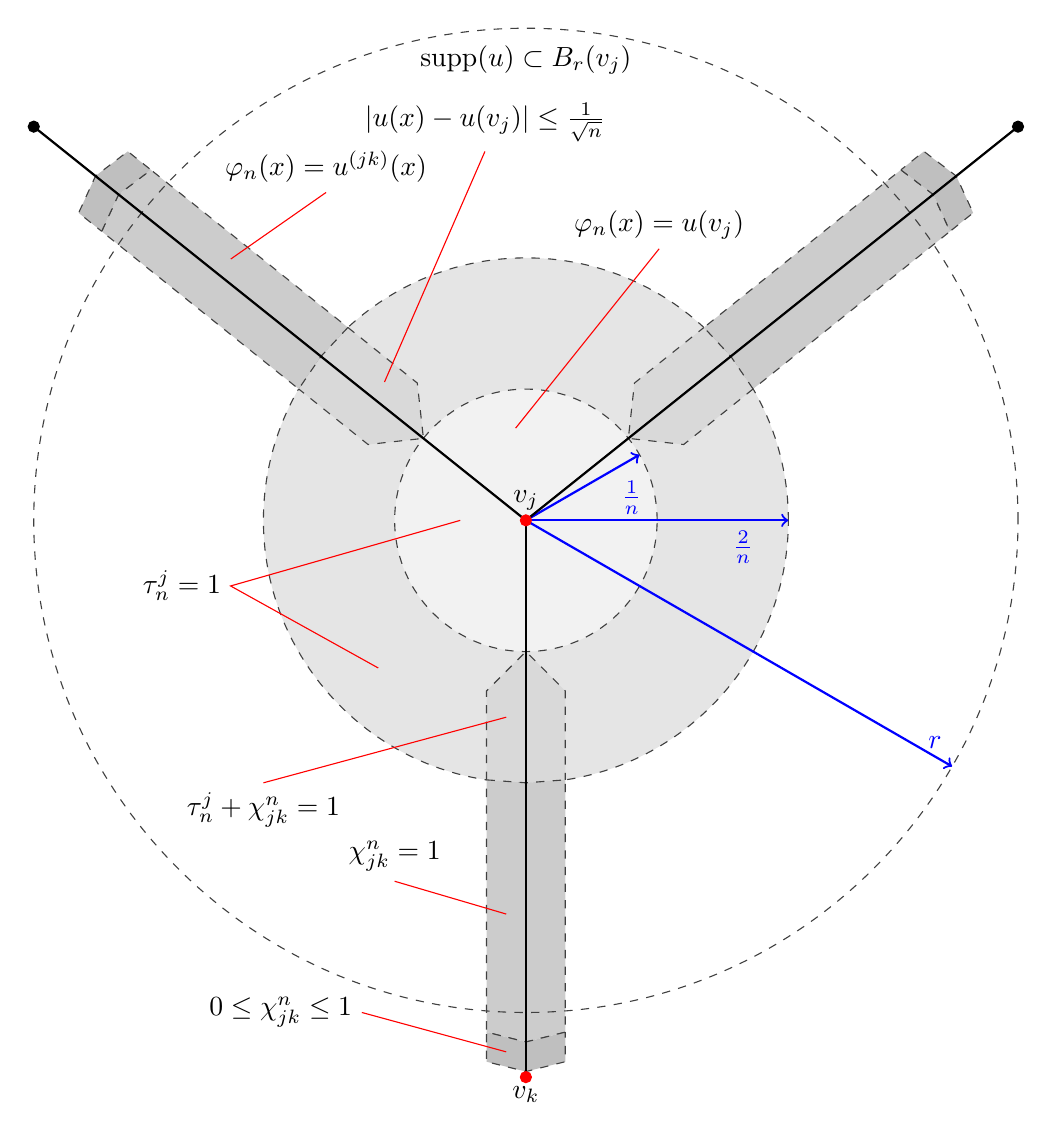
\begin{tikzpicture}[]

	% length of edges to rescale plots if needed
	\def\l{5}
	% coordinates for the vertices
	\coordinate (vc) at (0,0);
	\coordinate (v1) at (-1.25*\l,\l);
	\coordinate (v2) at (1.25*\l,\l);
	\coordinate (v3) at (0,-{sqrt(\l*\l+\l*\l)});
	
	%macro to draw the hideous support shapes
	\newcommand{\chiSupp}{
		% support of edge functions \chi_{jk}^n intersecting support of \tau_n^j
		\fill[black!15!white] (-0.5,-1.3*\l/3) -- (0,-1*\l/3) -- (0.5,-1.3*\l/3) -- (0.5, -{sqrt(4*\l*\l/9-0.25)}) -- (0,-2*\l/3) -- (-0.5, -{sqrt(4*\l*\l/9-0.25)}) -- cycle;
		\draw[draw=black!75!white, dashed] (-0.5, -{sqrt(4*\l*\l/9-0.25)}) -- (-0.5,-1.3*\l/3) -- (0,-1*\l/3) -- (0.5,-1.3*\l/3) -- (0.5, -{sqrt(4*\l*\l/9-0.25)});
		
		% remaining region of edge functions \chi_{jk}^n=1
		\filldraw[black!20!white, draw=black!75!white, dashed] (-0.5, -{sqrt(4*\l*\l/9-0.25)}) -- (0,-2*\l/3) -- (0.5, -{sqrt(4*\l*\l/9-0.25)}) -- (0.5,-1.3*\l) -- (0,-1.325*\l) -- (-0.5,-1.3*\l) -- cycle;
		
		% remaining support of the edge functions
		\filldraw[black!25!white, draw=black!75!white, dashed] (0.5,-1.3*\l) -- (0,-1.325*\l) -- (-0.5,-1.3*\l) -- (-0.5,-1.375*\l) -- (0,-1.4*\l) -- (0.5,-1.375*\l) -- cycle;
	}

	%DRAW LAYERS BACKWARDS DON'T FORGET!

	% balls of radius 1/n and 2/n
	\filldraw[black!10!white, draw=black!75!white, dashed] (vc) circle (2*\l/3); % node[anchor=center, align=center, color=black] at (0,\l/2) {$\varphi_n(x)=u(v_j)$};
	\filldraw[black!5!white, draw=black!75!white, dashed] (vc) circle (\l/3);% node[anchor=center, align=center, color=black] at (0,0.5*\l/3) {$\varphi_n(x)=u(v_j)$};

	% support for lower edge
	\chiSupp
	% support for top-left edge
	\begin{scope}[rotate around={180+atan(1.25):(vc)}]
		\chiSupp	
		% label values of the smooth approximating functions
		\draw[red] (-0.25,-1.5*\l/3) -- (-2*\l/3,-2*\l/3) node[anchor=south, align=center, color=black] {$\left\vert u(x)-u(v_j) \right\vert \leq \frac{1}{\sqrt{n}}$};
		\draw[red] (-\l/6,-\l/6) -- (-0.75*\l,-0.5*\l/3) node[anchor=south, align=center, color=black] {$\varphi_n(x)=u(v_j)$};
		\draw[red] (-0.25,-1.5*2*\l/3) -- (-1*\l/3,-2.75*\l/3) node[anchor=south, align=center, color=black] {$\varphi_n(x)=u^{(jk)}(x)$};
	\end{scope}
	\begin{scope}[rotate around={180+atan(-1.25):(vc)}]
		\chiSupp
	\end{scope}

	% ball of radius r containing support of function
	\draw[dashed, black!75!white] (vc) circle (1.25*\l) node[anchor=north, align=center, color=black] at (0, 1.25*\l-0.1) {$\mathrm{supp}(u)\subset B_r(v_j)$};
	% size of balls with arrows
	\draw[->, thick, blue] (vc) -- ({\l/3*cos(30)},{\l/3*sin(30)}) node[anchor=north west] at ({0.75*\l/3*cos(30)},{0.75*\l/3*sin(30)}) {$\frac{1}{n}$};
	\draw[->, thick, blue] (vc) -- ({2*\l/3*cos(0)},{2*\l/3*sin(0)}) node[anchor=north west] at ({0.75*2*\l/3*cos(0)},{0.75*2*\l/3*sin(0)}) {$\frac{2}{n}$};
	\draw[->, thick, blue] (vc) -- ({1.25*\l*cos(-30)},{1.25*\l*sin(-30)}) node[anchor=south east] at ({1.25*\l*cos(-30)},{1.25*\l*sin(-30)+0.1}) {$r$};

	% label partitions of unity
	\draw[red] (-0.25,-1.5*\l/3) -- (-2*\l/3,-2*\l/3) node[anchor=north, align=center, color=black] {$\tau_n^j+\chi_{jk}^n=1$};
	\draw[red] (-0.25,-1.5*2*\l/3) -- (-1*\l/3,-2.75*\l/3) node[anchor=south, align=center, color=black] {$\chi_{jk}^n=1$};
	\draw[red] (-0.25,-1.35*\l) -- (-1.25*\l/3,-1.25*\l) node[anchor=east, align=center, color=black] {$0\leq\chi_{jk}^n\leq1$};
	\draw[red] (-\l/6,0) -- (-0.75*\l,-0.5*\l/3) node[anchor=east, align=center, color=black] {$\tau_n^j=1$} -- (-0.75*\l/2,-0.75*\l/2);

	%DRAW GRAPH OBJECTS LAST, OVER THE TOP OF EVERYTHING
	% draw edges
	\draw[black, thick] (vc) -- (v1);
	\draw[black, thick] (vc) -- (v2);
	\draw[black, thick] (vc) -- (v3);

	% draw vertices
	\filldraw[red] (vc) circle (2pt) node[anchor=south, color=black] {$v_j$};
	\filldraw (v1) circle (2pt);
	\filldraw (v2) circle (2pt);
	\filldraw[red] (v3) circle (2pt) node[anchor=north, color=black] {$v_k$};

\end{tikzpicture}
\end{document}